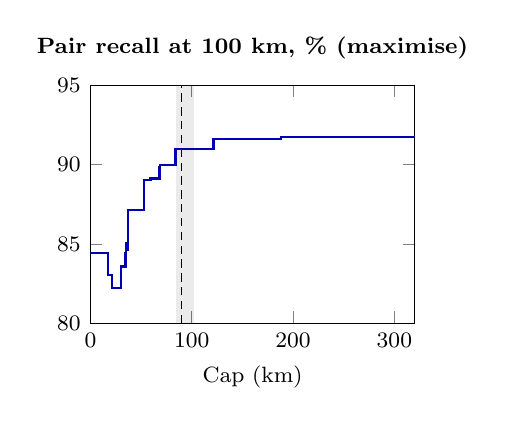
\begin{tikzpicture}
\begin{axis}[width=0.47\linewidth,height=4.6cm,xmin=0,xmax=320,ymin=80,ymax=95,title={Pair recall at 100 km, \% (maximise)},xlabel={Cap (km)},tick label style={font=\footnotesize},label style={font=\footnotesize},title style={font=\footnotesize\bfseries}]
\fill[black,opacity=0.08] (axis cs:84.06,80) rectangle (axis cs:102.47,95);
\draw[black,densely dashed] (axis cs:90,80) -- (axis cs:90,95);
\addplot[const plot mark left,thick,blue!70!black,no markers] coordinates {(0.00,84.4142) (12.80,84.4142) (17.36,83.0544) (17.67,83.0544) (19.38,83.0544) (19.45,83.0544) (19.91,83.0544) (20.85,83.0544) (21.31,82.2176) (22.89,82.2176) (23.13,82.2176) (23.51,82.2176) (25.04,82.2176) (25.47,82.2176) (28.92,82.2176) (29.68,82.2176) (30.15,83.5774) (31.07,83.5774) (34.15,83.5774) (34.27,83.5774) (34.69,84.4142) (34.82,85.0418) (34.95,84.6234) (36.35,84.6234) (36.70,87.1339) (40.41,87.1339) (44.07,87.1339) (47.75,87.1339) (52.59,89.0167) (59.32,89.1213) (68.26,89.8536) (68.84,89.9582) (84.06,91.0042) (101.37,91.0042) (102.47,91.0042) (110.59,91.0042) (111.08,91.0042) (117.62,91.0042) (121.52,91.6318) (121.69,91.6318) (122.12,91.6318) (122.76,91.6318) (125.71,91.6318) (131.64,91.6318) (132.45,91.6318) (139.11,91.6318) (142.83,91.6318) (142.86,91.6318) (146.10,91.6318) (149.97,91.6318) (154.64,91.6318) (157.99,91.6318) (165.66,91.6318) (165.79,91.6318) (170.37,91.6318) (176.07,91.6318) (178.09,91.6318) (183.33,91.6318) (186.70,91.6318) (188.07,91.6318) (188.38,91.7364) (191.88,91.7364) (192.60,91.7364) (193.28,91.7364) (320.00,91.7364)};
\end{axis}
\end{tikzpicture}\hfill
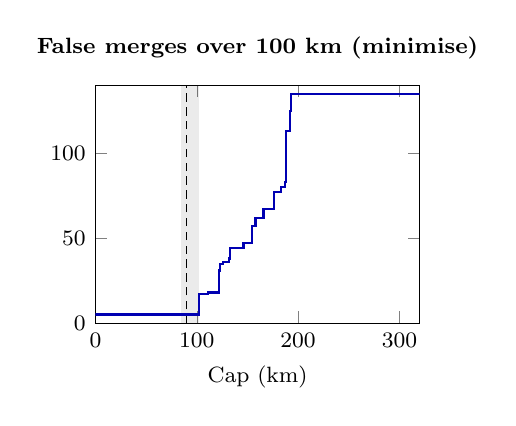
\begin{tikzpicture}
\begin{axis}[width=0.47\linewidth,height=4.6cm,xmin=0,xmax=320,ymin=0,ymax=140,title={False merges over 100 km (minimise)},xlabel={Cap (km)},tick label style={font=\footnotesize},label style={font=\footnotesize},title style={font=\footnotesize\bfseries}]
\fill[black,opacity=0.08] (axis cs:84.06,0) rectangle (axis cs:102.47,140);
\draw[black,densely dashed] (axis cs:90,0) -- (axis cs:90,140);
\addplot[const plot mark left,thick,blue!70!black,no markers] coordinates {(0.00,5.0000) (12.80,5.0000) (17.36,5.0000) (17.67,5.0000) (19.38,5.0000) (19.45,5.0000) (19.91,5.0000) (20.85,5.0000) (21.31,5.0000) (22.89,5.0000) (23.13,5.0000) (23.51,5.0000) (25.04,5.0000) (25.47,5.0000) (28.92,5.0000) (29.68,5.0000) (30.15,5.0000) (31.07,5.0000) (34.15,5.0000) (34.27,5.0000) (34.69,5.0000) (34.82,5.0000) (34.95,5.0000) (36.35,5.0000) (36.70,5.0000) (40.41,5.0000) (44.07,5.0000) (47.75,5.0000) (52.59,5.0000) (59.32,5.0000) (68.26,5.0000) (68.84,5.0000) (84.06,5.0000) (101.37,5.0000) (102.47,17.0000) (110.59,17.0000) (111.08,18.0000) (117.62,18.0000) (121.52,18.0000) (121.69,26.0000) (122.12,31.0000) (122.76,35.0000) (125.71,36.0000) (131.64,38.0000) (132.45,44.0000) (139.11,44.0000) (142.83,44.0000) (142.86,44.0000) (146.10,47.0000) (149.97,47.0000) (154.64,57.0000) (157.99,62.0000) (165.66,62.0000) (165.79,67.0000) (170.37,67.0000) (176.07,77.0000) (178.09,77.0000) (183.33,80.0000) (186.70,83.0000) (188.07,103.0000) (188.38,113.0000) (191.88,125.0000) (192.60,134.0000) (193.28,135.0000) (320.00,135.0000)};
\end{axis}
\end{tikzpicture}

\medskip
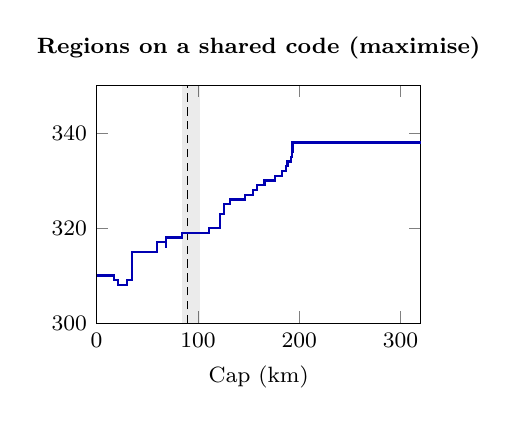
\begin{tikzpicture}
\begin{axis}[width=0.47\linewidth,height=4.6cm,xmin=0,xmax=320,ymin=300,ymax=350,title={Regions on a shared code (maximise)},xlabel={Cap (km)},tick label style={font=\footnotesize},label style={font=\footnotesize},title style={font=\footnotesize\bfseries}]
\fill[black,opacity=0.08] (axis cs:84.06,300) rectangle (axis cs:102.47,350);
\draw[black,densely dashed] (axis cs:90,300) -- (axis cs:90,350);
\addplot[const plot mark left,thick,blue!70!black,no markers] coordinates {(0.00,310.0000) (12.80,310.0000) (17.36,309.0000) (17.67,309.0000) (19.38,309.0000) (19.45,309.0000) (19.91,309.0000) (20.85,309.0000) (21.31,308.0000) (22.89,308.0000) (23.13,308.0000) (23.51,308.0000) (25.04,308.0000) (25.47,308.0000) (28.92,308.0000) (29.68,308.0000) (30.15,309.0000) (31.07,309.0000) (34.15,309.0000) (34.27,309.0000) (34.69,310.0000) (34.82,313.0000) (34.95,315.0000) (36.35,315.0000) (36.70,315.0000) (40.41,315.0000) (44.07,315.0000) (47.75,315.0000) (52.59,315.0000) (59.32,317.0000) (68.26,316.0000) (68.84,318.0000) (84.06,319.0000) (101.37,319.0000) (102.47,319.0000) (110.59,319.0000) (111.08,320.0000) (117.62,320.0000) (121.52,321.0000) (121.69,322.0000) (122.12,323.0000) (122.76,323.0000) (125.71,325.0000) (131.64,326.0000) (132.45,326.0000) (139.11,326.0000) (142.83,326.0000) (142.86,326.0000) (146.10,327.0000) (149.97,327.0000) (154.64,328.0000) (157.99,329.0000) (165.66,329.0000) (165.79,330.0000) (170.37,330.0000) (176.07,331.0000) (178.09,331.0000) (183.33,332.0000) (186.70,333.0000) (188.07,333.0000) (188.38,334.0000) (191.88,335.0000) (192.60,336.0000) (193.28,338.0000) (320.00,338.0000)};
\end{axis}
\end{tikzpicture}\hfill
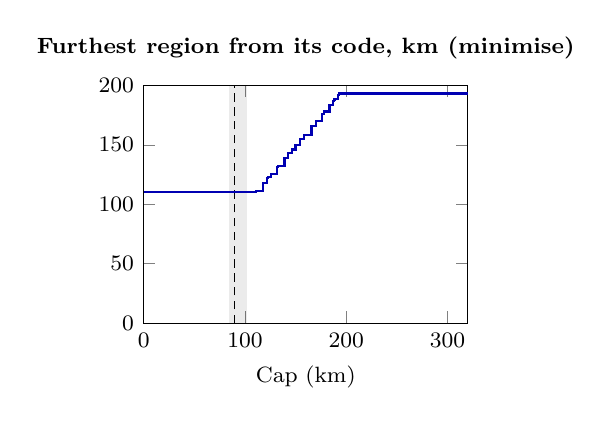
\begin{tikzpicture}
\begin{axis}[width=0.47\linewidth,height=4.6cm,xmin=0,xmax=320,ymin=0,ymax=200,title={Furthest region from its code, km (minimise)},xlabel={Cap (km)},tick label style={font=\footnotesize},label style={font=\footnotesize},title style={font=\footnotesize\bfseries}]
\fill[black,opacity=0.08] (axis cs:84.06,0) rectangle (axis cs:102.47,200);
\draw[black,densely dashed] (axis cs:90,0) -- (axis cs:90,200);
\addplot[const plot mark left,thick,blue!70!black,no markers] coordinates {(0.00,110.4387) (12.80,110.4387) (17.36,110.4387) (17.67,110.4387) (19.38,110.4387) (19.45,110.4387) (19.91,110.4387) (20.85,110.4387) (21.31,110.4387) (22.89,110.4387) (23.13,110.4387) (23.51,110.4387) (25.04,110.4387) (25.47,110.4387) (28.92,110.4387) (29.68,110.4387) (30.15,110.4387) (31.07,110.4387) (34.15,110.4387) (34.27,110.4387) (34.69,110.4387) (34.82,110.4387) (34.95,110.4387) (36.35,110.4387) (36.70,110.4387) (40.41,110.4387) (44.07,110.4387) (47.75,110.4387) (52.59,110.4387) (59.32,110.4387) (68.26,110.4387) (68.84,110.4387) (84.06,110.4387) (101.37,110.4387) (102.47,110.4387) (110.59,110.5943) (111.08,111.0803) (117.62,117.6153) (121.52,121.5183) (121.69,121.6887) (122.12,122.1152) (122.76,122.7610) (125.71,125.7067) (131.64,131.6389) (132.45,132.4543) (139.11,139.1144) (142.83,142.8344) (142.86,142.8619) (146.10,146.0988) (149.97,149.9715) (154.64,154.6437) (157.99,157.9948) (165.66,165.6552) (165.79,165.7942) (170.37,170.3664) (176.07,176.0716) (178.09,178.0854) (183.33,183.3345) (186.70,186.6972) (188.07,188.0684) (188.38,188.3797) (191.88,191.8822) (192.60,192.5966) (193.28,193.2778) (320.00,193.2778)};
\end{axis}
\end{tikzpicture}
